\section{Dataset}
\label{sec:dataset}

\subsection{Data Description}

Our models use six datasets: HDB flats, HDB blocks, MRT stations, schools, shopping malls, and hawker centres. The first five are in structured CSV formats, while the last is in GeoJSON, obtained from Singapore's government open data portal. COE prices and share prices were also tested and rejected (Section~\ref{sec:level-results}). All other files come from the course competition \cite{CS5228:2026:Malls}.

The core dataset contains 200,000 records on ten features of HDB flats and one target: the monthly flat rent. The records describe approved rental applications in Singapore, down to the block level but with individual unit numbers omitted. These are recorded at monthly granularity with no specific day provided, spanning from Jan 2021 to Jul 2026. Related public data are published by HDB \cite{HDB:2026:Rentals, HDB:2026:Blocks}, the Land Transport Authority \cite{LTA:2024:MRT}, the Ministry of Education \cite{MOE:2026:Schools} and the National Environment Agency \cite{NEA:2026:Hawkers}, although the competition files carry extra columns such as coordinates. The auxiliary datasets supplement the core dataset, and their incorporation is discussed below. In total, our tuned baseline uses 19 features: six from the core dataset and 13 block-level features. The final model adds three more built from each block's past rentals.


\subsection{Data Preprocessing}

The split of the train and test sets is temporal: the train set covers records from Jan 2021 to Mar 2025, and the test set covers the remaining records from Mar 2025 to Jul 2026. Only 380 test records (0.76\%) share a month with the train set. This corresponds to a train-test split of 75-25. The temporal split motivates many of our decisions in the sections that follow (Fig.~\ref{fig:timeline}).

\begin{figure}[htbp]
\centerline{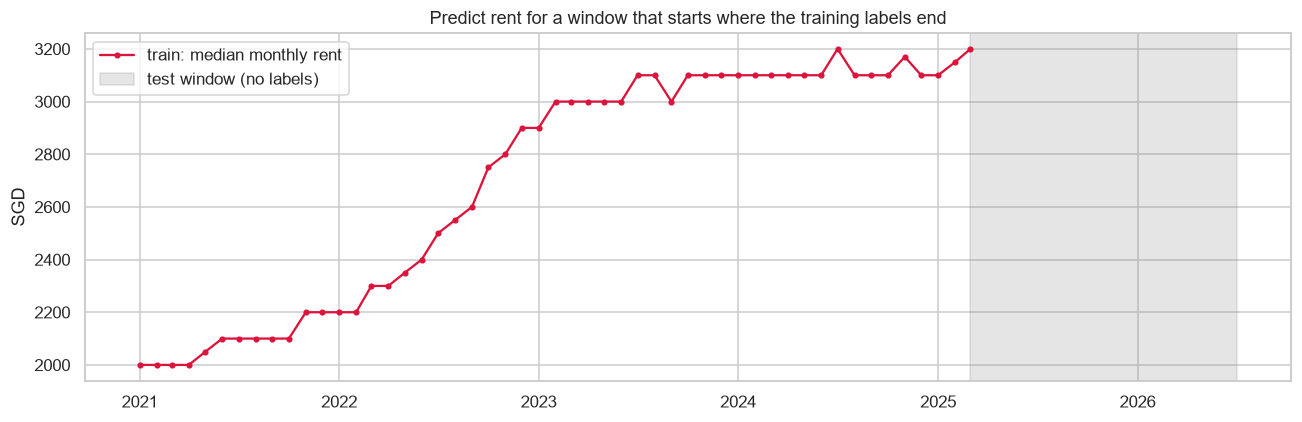
\includegraphics[width=\columnwidth]{figures/train_test_timeline.png}}
\caption{Median monthly rent in the train set. The test window starts where the labels end.}
\label{fig:timeline}
\end{figure}

For the core dataset, two issues required cleaning. First is the inconsistent hyphenation of the flat\_type feature (e.g., “4-room” and “4 room”). These are all normalized to their hyphenated counterparts, thereby reducing the cardinality from 11 to 6. Second is the inconsistent casing of the street feature, so all values are set to lowercase which reduces its cardinality from 1146 to 576.

Each record is tracked by a datetime feature, however, most models cannot directly interpret datetime values. To address this, we transform the feature into a numerical variable called month\_index, representing the index of the observed month relative to the first observation's (e.g. 2021-01 has index 0, 2021-02 has index 1, etc.).

LightGBM takes town, flat type and flat model as native categorical features, with levels fixed from the training data, and handles missing building heights natively (11 blocks, 159 training rows, none in test). The GNN and its MLP control one-hot encode their categorical features, and median-impute and standardise their numeric features with a missing-value indicator, all fitted on the training rows only.

Two features contain only constant values, namely: furnished and fee. As they provide no useful information for prediction and to reduce dataset size, both features were dropped. Histograms and box plots of the remaining numerical features (Fig.~\ref{fig:eda}) show 752 rents (0.50\%) and 130 floor areas beyond the 1.5 IQR whiskers. Rents run from \$300 to \$7,600. We have no evidence that these are errors, so we kept them. There are no missing values, though a few exact duplicate records for HDB rentals were found, representing 425 records (0.28\% of the train set). While seemingly alarming, these duplicates may reflect real records. As the dataset covers HDB flats at the block level with monthly granularity, it is possible that different units of the same flat type were rented at the same block within the same month. Therefore, our verdict is to keep these duplicates.

For the auxiliary datasets, preprocessing was performed separately for HDB blocks, MRT stations, and schools. For HDB blocks, the town, block, and street were lowercased and stripped of surrounding whitespace, achieving a 100\% match with rental records in both training and test sets. Values of $-1$ in max\_floor and year\_completed were converted to missing values for 11 blocks. Among their 159 training rental records, 115 (72.3\%) corresponded to three-room flats in Clementi. These are older blocks with no test records, and dropping them made almost no difference once building height was in the model, so all 159 records were kept. 

For MRT stations, operational stations were selected and deduplicated by station name before feature generation to prevent interchanges from being counted multiple times across lines. The interchange flag comes from the source and includes nine stations that are only planned to become interchanges. For schools, coordinates for eight records were updated after checks against school addresses and referenced MRT stations. These updates corrected locations associated with similarly named schools or outdated campuses and refined imprecise positions, improving the accuracy of nearest-school distances and school counts within the selected radii.


\subsection{Exploratory Data Analysis}

% Factors such as flat type, location, and nearby amenities, alongside broader economic conditions, can directly influence the demand for HDB flats and their rental prices.

Over the training period, rents were observed to increase by 56\% in two regimes: a climb to mid-2023, then a flat market. Time correlates most with rent (Spearman 0.56), followed by floor area (0.32) and lease commencement year (0.23). There is no usable seasonality (under 2\%), so we add no month-of-year feature. Due to the temporal split of the train and test sets, the target moves over time as well; thus, our validation is also on time-ordered splits. Floor area, lease year and flat type shares do not drift materially between the train and test sets. Floor area and flat type correlate at 0.95, but keeping both would perform better than either alone, so both features were kept.

Location is widely cited as a main factor in rental price \cite{Poh:2023:Location}, which motivates the auxiliary datasets. In our data, median rent runs from \$1,450 for 1-room to \$3,000 for executive flats, against only \$2,500 to \$3,000 across the 26 towns (Fig.~\ref{fig:eda}), so town alone captures little of location. We use the dataset for HDB blocks to attach coordinates to flats in the main dataset which are joined on the town, block, and street features. Afterwards, using the Haversine formula, we compare each HDB block’s coordinates with those of operational MRT stations, schools, shopping malls, and hawker centres that are not under construction to derive their straight-line distance in kilometers.  Multiple features were then created which count the number of each amenity type within varying radii (i.e., 500 m, 1 km, 2 km).

Additionally, we calculate the distances of the HDB blocks to (1) nearby amenities and (2) Raffles Place MRT station. First, amenities refer to nearby primary schools, operational MRT stations, MRT interchanges, shopping malls, and hawker centres. Amenity counts describe the density of these nearby facilities, but do not distinguish how close the nearest facility is, so we also compute their distances. Second, Raffles Place MRT station is used as a fixed reference point for CBD proximity, since Raffles Place is one of the core areas of Singapore's CBD \cite{URA:2026:CBD}. Together, the amenity counts, distances to the nearest facilities, and distance to Raffles Place MRT station capture both the availability of nearby amenities and their proximity, as well as proximity to Singapore's CBD. We tested these sets by their RMSE on the holdout period of Section~\ref{sec:holdout}, keeping a set that lowered it from 496.4 on the base columns to 489.6. Since the features were selected based on this holdout period, the improvement is somewhat optimistic. We excluded the block's year of completion, which worsened RMSE, and area-level school and MRT totals, which worsened it alone and added only 0.4 on top of block-level features, for eight extra columns. Thus, the final set consists of 13 block-level features, containing building height, counts within 2 km for primary schools and MRT stations, counts within 1 km for secondary schools, MRT interchanges, shopping malls and hawker centres, the nearest distances to primary schools, MRT stations, MRT interchanges, malls and hawker centres, and the distance to the CBD.


An additional feature for flat age is generated, the reasons for which are twofold. First, age and upkeep may affect rent \cite{Eng:2022:Factors}. Second, mature estates tend to command higher rents with better-established amenities \cite{Poh:2023:Location}. Flat age and lease commencement year carry nearly the same information for a given month, so our main LightGBM models use the lease year directly, while flat age is used for the market-level regression and neural models. The block and street are used to identify each flat's location but are not included directly as model features; instead, block-specific historical effects are captured through the premiums described in Section~\ref{sec:lightgbm}.


% Exploratory Data Analysis \& Preprocessing. Explain and justify your approach to understand the data, and how it informed your data preprocessing steps (e.g., data reduction, data transformation, outlier removal, feature generation).
